\infolevone{
\subsection{SHMS Aerogel Detector}

The SHMS Aerogel detector \cite{HornSHMSAerogel} is located after the Heavy Gas Cherenkov
detector and before the S2 hodoscope planes.  It provides kaon/proton
discrimination up to 7.2 $\textrm{GeV}/c$.  The detector is mounted on
a sliding rail system so that it may easily be placed into or removed
from the path of particles in the detector hut.  Several Aerogel
indices of refraction, shown in Table~\ref{tab:shms_aerogel}, are
available for use with the detector.  The material in the path of
particles passing through the detector stack is sumarized in
Table~\ref{tab:shms_aerogelmaterial}.

\begin{table}
\caption{Momentum threshold above which pions, kaons and protons will
produce Cherenkov light in Aerogels with various indices of refraction.
\label{tab:shms_aerogel}}
\begin{center}
\begin{tabular}{cccc}
  n& $\pi_{\textrm{thr}}(\textrm{GeV}/c)$ & $K_{\textrm{
  thr}}(\textrm{GeV}/c)$ & $p_{\textrm{thr}}(\textrm{GeV}/c)$\\
  1.030 & 0.57 & 2.00 & 3.80 \\
  1.020 & 0.67 & 2.46 & 4.67 \\
  1.015 & 0.81 & 2.84 & 5.40 \\
  1.011 & 0.94 & 3.32 & 6.31 \\
\end{tabular}
\end{center}
\end{table}

\newcommand{\specialcell}[2][c]{%
  \begin{tabular}[#1]{@{}c@{}}#2\end{tabular}}

\begin{table}
\caption{List of  materials in the path of particles traversing the SHMS
  aerogel detector
\label{tab:shms_aerogelmaterial}}
\begin{center}
\begin{tabular}{ccccc}
Component & Material &\specialcell{Thickness\\(cm)}
& \specialcell{Density\\$(\textrm{g}/\textrm{cm}^3)$}
& \specialcell{Radiation Length\\$(\textrm{g}/\textrm{cm}^2)$}\\
Entrance Window & Al & 0.13 & 2.7 & 24.01 \\
Aerogel & $\textrm{SiO}_2$ & 9 & 0.2 &  44.054 \\
Air gap in detector & Air & 17.1 & 0.00121 & 36.66 \\
Exit window & Al &  0.16 & 2.7 & 24.01  \\
\end{tabular}
\end{center}
\end{table}

\subsubsection{Design Overview}

The detector consists of two main components: a tray
which holds the aerogel material, and a light diffusion box with
photomultiplier tubes (PMTs) for light readout. To cover the required
kaon identification momentum range of up to 7.2 $\textrm{GeV}/c$, four identical
trays for aerogel of nominal refractive indices of 1.030, 1.020,
1.015, and 1.011 were constructed. Using 5-inch diameter PMTs mounted
on the vertical sides of the diffusion box and up to 9 cm aerogel
thickness in the trays, the total depth of the detector is 29.0 cm
along the optical axis of the SHMS. The design allows for replacement
of the aerogel trays.


The main components and features of the detector assembly are:
\begin{itemize}
  \item \textbf{Diffusion box} made mostly of aluminum alloy 6061-T6. The
    sides and top panel are constructed of 2.5 cm (1-inch) aluminum
    plates, while the bottom plate is made of a 1 inch stainless steel
    plate. The back cover is 1.6 mm (1/16 inch) thick aluminium. The
    inner dimensions of the box are $113\times 103
times 17.3~\textrm{cm}^3$ ($44.5\times 40.5\times 6.75~\textrm{inch}^3$).
  \item \textbf{Four (4) exchangeable aerogel trays}, of the same transverse
    size as the diffusion box but 11.3 cm (4.45 inch) deep. The front
    cover of the trays is made of a 5 mm thick honeycomb sandwich
    panel with effective aluminum thickness of 1.3 mm (0.050 inch).
  \item \textbf{Fourteen (14) 5-inch diameter photo-multiplier tubes}
    (Photonis XP4572B) mounted upon waterjet cut circular openings on
    the left and right sides of the diffusion box. The mechanical
    design includes six openings on the top of the diffusion box,
    presently covered with blanks. PMTs are placed in aluminum
    cylinders for mechanical protection, with a 1mm thick mu-metal
    cylinder (also inside the aluminum cylinder) for magnetic
    shielding.
  \item \textbf{Fourteen (14) positive HV active bases}   These
  bases include built-in amplifiers powered by the voltage
  divider~\cite{Popov2001,Popov2003316}.
  \item \textbf{Approximately 700 tiles of aerogel ($\unsim 10$ kg) installed in each
    tray} in a running break bond pattern. Total thickness of the
    aerogel radiator along the optical axis is $\unsim 9$ cm, or 8 tiles. Each
    tile has approximate dimensions of 11 cm by 11 cm by 1.1 cm.
  \item \textbf{GORE reflector material} (DRP-1.0-12x30-PSA) with reflectivity
    of about 99\% covering the inner surface of the diffusion box with
    3 mm ($\sim$60\% of the surface) and 1 mm ($\sim$40\% of the surface)
    thickness.
  \item \textbf{Millipore paper Membrane GSWP-0010} of reflectivity of $\unsim 96\%$
    covering the inner surface of the SP-30 and SP-20 aerogel trays
    with 1 layer of 0.45 $\mu$m thickness.
  \begin{itemize}
    \item 1 mm thick Gore diffusive reflector material is used instead
      of Millipore in the two lower refractive index trays (SP-15 and
      SP-11) to optimize light collection.
  \end{itemize}
  \item \textbf{Aluminum mounting hardware}.
\end{itemize}
The aerogel trays attach to the diffusion box by means of bolting
(stainless steel $\textrm{\#10-24UNC}\times 0.63$ inch length hex tap bolts) through
flanges surrounding the boxes. A round O-ring (1/8 inch EDPM of $\unsim 175$
inch
length – cut to size) runs in the flange groove around the diffusion
box and ensures light tight connection. Additionally, Scotch 130C tape
is added on the top of the O-ring for light tightness of the
detector. The entire detector is designed such that it can be slid out
of the SHMS detector stack for aerogel tray exchange. Note, however,
that no experiment can run with detector in this position since the
right-side PMTs will extend into the SHMS acceptance.

\subsubsection{Installation Location and General Operating Procedures}
The SHMS aerogel detector is installed in the detector hut of the SHMS
between the heavy gas Cherenkov and the second hodoscope plane. The
installation and/or removal of the SHMS Aerogel Detector must be
handled by Hall C technical staff, with experts’ assistance (see list
of experts at the end). In general, the detector is designed for
removal from the sliding detector stand.

Prior to any work that involves exchange of the aerogel trays or
installation/removal of the diffusion box, the plastic safety cover on
the Heavy Gas Cherenkov must be installed. This cover must be removed
before resuming regular operation.

Before moving the diffusion box it should be checked that all high
voltage and signal cables are long enough for the move or are
disconnected from the HV bases. After any move of the detector it
should be verified that the center of the aerogel detector is aligned
with the SHMS optics axis. This should follow automatically when the
detector is mounted on its stand and slides in its nominal
position. Nevertheless, a survey should be performed after any major
move of the detector. The drawings of the detector and its stand are
available from the Hall C engineering group.

The photomultiplier tubes and bases are operated at positive high
voltages up to $\unsim 2000$ V (see Table~\ref{tab:shms_aerogelhv}). No directly accessible
components carry high voltage. Standard safety precautions for
handling high voltage on photo tubes must be observed, including, but
not limited to disabling the HV at the power supply and disconnecting
the HV cables from the bases (except in limited test cases) whenever
the base covers are removed (to avoid electrical shock), or whenever
there is possibility of room light entering the aerogel box (to avoid
damaging photo-cathodes of the tubes). The personnel shall be careful
when removing a tube-base assembly, shall avoid mechanical shocks of
the tubes and of the whole assembly in order not to break the glass
tubes and to preserve the properties of the inner mu-metal shielding.

The composition of the aerogel material is
$(2n(\textrm{SiO}_2)+2n(\textrm{H}_2 \textrm{O})+\textrm{air})$. This type of aerogel is not hygroscopic and
will not loose its detector capabilities if contaminated with vapors
from air. But, the box should be kept sealed whenever possible, clean
and dry, and the material should not be touched directly. The aerogel
is rather fragile, and a tile (especially of the lowest index of
refraction $n=1.011$) will usually not support its weight when grasped
with one hand.

None of the materials and components used are known to pose any health
or environmental hazards beyond cutting skin from broken glass or
sharp edges. Any debris (dust) from a damaged aerogel material can be
wiped off with a damp cloth or washed off. Extreme care should be
taken to avoid getting aerogel dust or fragments in the eyes. Seek
medical attention if this occurs.

The aerogel box, including aerogel material and tube/base assemblies
but excluding SHMS mounting hardware, weighs about 100 kg and can be
handled by 4 persons during (de-) installation.

\subsubsection{Aerogel Tray Exchange}
Installation and/or removal of the SHMS Aerogel Cherenkov must be
handled by Hall C technical staff, with experts’ assistance (see
list of experts at the end). Following is the standard procedure for
change of aerogel tray:

\subsubsection*{Preparations}

\begin{itemize}
  \item turn off HV voltage on the aerogel Cherenkov detector, and on
    all nearby detectors (in special the Heavy Gas Cherenkov and the
    hodoscope);
  \item be sure that you and detectors are protected from any
    accidental HV connections;
  \item watch the HV and signal cables on the diffusion box during any
    movement of the detector. Removal may not be necessary
  \item install the plastic cover on the window of Heavy Gas Cherenkov on the
    aerogel tray side, i.e., downstream of the aerogel detector;
  \item mark current position of the aerogel detector in the detector
    stand (detector and components must be placed back at exact same
    position);
  \item keep all tools ready: mechanical supports and necessary
    materials which you will need for this operation (wrenches of
    different sizes, alignment pins, a spare O-ring, support
    structure, black tape, plastic cover for the Heavy Gas Cherenkov,
    cover for empty box while tray is being exchanged);
  \item taking out an aerogel tray from detector hut or replacing an
    aerogel tray requires a specially designed support structure (look
    in the physics storage building or ask the Hall C coordinator).
    \end{itemize}

\textbf{NEVER APPLY FORCE TO A PMT OR DETECTOR
  FRONT WINDOW!  AVOID MECHANICAL SHOCKS OF THE DETECTOR DURING
  TRANSPORTATION \& INSTALLATION!  KEEP AEROGEL TRAY AT OPERATING ANGLE
  $\unsim 18$ DEGREES!}

\subsubsection*{Removal of an aerogel tray}

\begin{itemize}
  \item remove part of the roof of the SHMS hut (if that is in place),
    making enough room for lifting the aerogel tray in the horizontal
    position
  \item place a pallet on the floor of the SHMS hut for lifting the
    aerogel tray out of the hut
  \item loosen the clamps that are fixing detector position (one on
    the top of the detector and two on the slide stand);
  \item move the detector out from its position by sliding (along two
    slide stands);
  \item move support structure into the SHMS detector hut and adjust
    its position to hold aerogel radiator when it will be disconnected
    from the diffusion box;
  \item loosen all bolts that connect tray with diffusion box; when
    all detectors are installed, this operation may require the use of
    a step ladder to loosen bolts on the detector side closest to the
    SHMS wall.
  \item fit the support stand and fix it to the aerogel tray position
    at the same angle $\unsim 18$ degrees (the SHMS normal operational
    position), using straps to tight the support to the tray's
    handles;
  \item remove all bolts that connect tray with diffusion box;
  \item gradually slide support structure with aerogel tray backward
    in order to disconnect it from diffusion box;
  \item put temporary shielding (black plastic or Tedlar cover) on the
    open window of diffusion box to keep its volume clean and dark,
    and put cover on the aerogel tray to keep its volume clean;
  \item carefully lower the aerogel tray assembly (aerogel tray with
    support structure) horizontally on the SHMS hut floor onto the
    pallet – aerogel facing up. If the overhead crane is used, the
    tray must be guided by hand to minimize shifting of the aerogel
    tiles, in particular for the lowest aerogel indices.
  \item secure the aerogel tray assembly to the pallet
  \item cover the aerogel tray with an aluminum plate
  \item take out aerogel tray assembly from the detector hut using the
    crane and always keeping the pallet in horizontal position;
  \item disconnect aerogel tray from support stand and put it on the
    floor (assuming you already have some flat soft material laid down
    on the floor);
  \item put all bolts and fix position of the cover on tray, put tape
    along the tray-cover contact line. (this should be before, still
    inside the hut, to avoid dirty material from the crane to
    contaminate the aerogel)
\end{itemize}

\subsubsection*{Installation of an aerogel tray (assume the new tray is
already in the SHMS balcony)}

\begin{figure}
\begin{center}
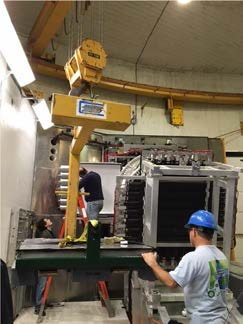
\includegraphics[width=3in]{shms-aerogel-1.jpg}
\caption{\label{fig:shms-aerogel-1}Aerogel tray on the pallet picked
  up by the crane.  }
\end{center}
\end{figure}

\begin{itemize}
  \item place the aerogel support structure onto a pallet that can be
    picked up by the crane
  \item place the aerogel tray horizontally with aerogel facing up
    onto the support structure on the pallet (see Fig.~\ref{fig:shms-aerogel-1})
  \item loosen bolts on cover and mount aerogel tray at the correct
    position on the support structure (use marks which indicate best
    position for joining aerogel tray with diffusion box). Secure the
    tray with a strap onto the support structure and pallet;
  \item  move the aerogel tray with support structure and pallet
    into the detector hut by use of the Hall C crane (keep the
    assembly horizontally);
  \item place the assembly on the SHMS hut floor. Unstrap the support
    and aerogel tray from the pallet.
  \item loosen bolts and, if installed, take away temporary covers
    from the aerogel tray and from the diffusion box;

\begin{figure}
\begin{center}
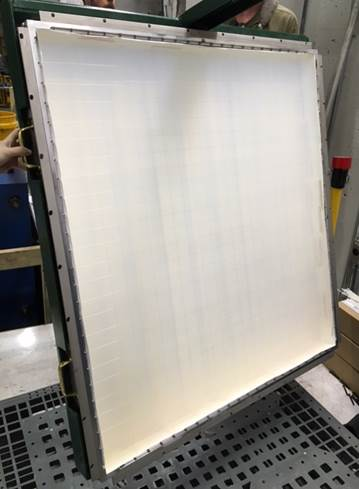
\includegraphics[width=3in]{shms-aerogel-2a.jpg}
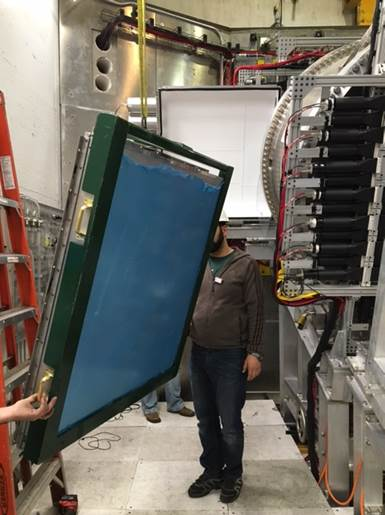
\includegraphics[width=3in]{shms-aerogel-2b.jpg}
\caption{\label{fig:shms-aerogel-2}Illustration of lifting the aerogel
  tray to 18 degrees by hand and lifting it at into position.}
\end{center}
\end{figure}

  \item Attach the support and aerogel assembly to the crane, but do
    not lift yet. First carefully lift the assembly by hand to the
    required 18 degree angle. Once that is done, carefully lift the
    tray (keep the assembly at 18 degrees angle) towards the diffusion
    box – this requires at least 2 people steadying the assembly
    during the lifting (see Fig.~\ref{fig:shms-aerogel-2})

\begin{figure}
\begin{center}
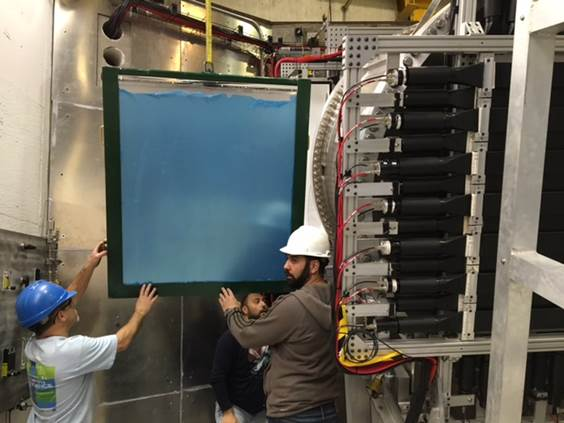
\includegraphics[width=3in]{shms-aerogel-3a.jpg}
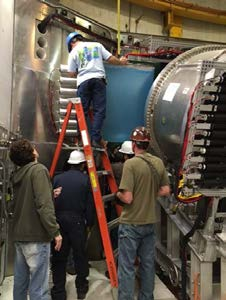
\includegraphics[width=3in]{shms-aerogel-3b.jpg}
\caption{\label{fig:shms-aerogel-3}Illustration of the alignment of
  the aerogel tray with the diffusion box.}
\end{center}
\end{figure}


  \item align position of the tray with the diffusion box. Make sure
    the flange O-ring is in place, make sure Scotch tape (C-130) is
    placed on top of O-ring, both in good conditions (otherwise
    replace them) (see Fig.~\ref{fig:shms-aerogel-3})
  \item insert 4-6 guide pins in the corners of diffusion box (to keep
    diffusion box and tray aligned);
  \item if all looks OK, move the aerogel tray gradually closer the
    diffusion box and try slide it into the inner border of the box;
  \item put all bolts and tighten them by hand; take out the guide
    pins and put remaining bolts; when tightening the bolts make sure
    to gradually tighten them from a variety of positions in order to
    distribute the force evenly and create a uniform seal.
\item Remove the support structure
\item once you're sure that
  everything is OK, tighten all the bolts gradually;
\item put a black
  scotch tape around connection line between the aerogel tray and
  diffusion box as an additional layer of protection against
  possible light leaks;
\item slide detector to its nominal position
  centered relative to the SHMS axis;
\item verify that the aerogel detector
  is in the correct position and fix it with clamps (one on the top
  of the detector and two on the slide stand);

\begin{figure}
\begin{center}
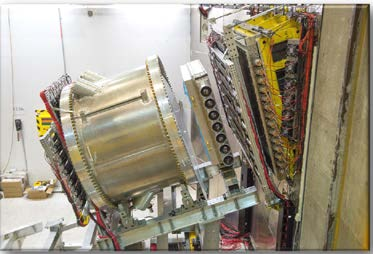
\includegraphics[width=3.5in]{shms-aerogel-4.jpg}
\caption{\label{fig:shms-aerogel-4}Kaon Aerogel detector in place at the SHMS detector hut.}
\end{center}
\end{figure}

\item make sure all HV and
  signal cables are properly connected;
\item switch HV ``ON'' for only one
  PMT and check for light leaks; start with a low HV of $\unsim 400-700$ V
  (lower than nominal operational HVs), check the PMT signals on
  oscilloscope;
\item switch HV ``ON'' for all PMTs and verify that no any
  light leak problem. Start again with an HV of $\unsim 400-700$ V (lower than
  the nominal operational HVs) and check the PMT signals on
  oscilloscope;
\item Once you are sure there is no light leak, ramp up all
  PMT HVs to their nominal values;
\item Remove the plastic cover from
  the window of Heavy Gas Cherenkov on the aerogel detector side;
\end{itemize}

\subsubsection{PMT Removal and Replacement}

The detector employs fourteen Photonis XP4572B PMTs. These are large
5'' diameter, 10 stage, bialkali photo-cathode tubes (flat glass
window). They are housed in cylinder shields.

\subsubsection*{PMT Removal}

\begin{itemize}
\item Make sure all HV’s are OFF!
\item Remember never touch or apply force to the photo-tube. The PMT
  window is very fragile!
\item Be sure that you and detector are
  protected from any accidental HV connections.
\item Disconnect signal
  and HV cables and remove the base.
\item Loosen 4 bolts that connect
  the housing cylinder with diffusion box.
\item Remove the entire
  photo-tube assembly
\item Install temporary shielding (plastic or Tedlar
  cover) on the open window to keep the detector volume clean.
\end{itemize}

\subsubsection*{PMT Replacement}

\begin{itemize}
\item Remember never touch or apply force to the photo-tube face. The
  PMT window is very fragile!  Place the flange on top of an
  ``office'' wastebasket with the aluminum cylinder pointing down.
\item Insert the O-ring into the  back of the wide part of the
  shield, slide the photo-tube in, and  place the plastic ring around
  the face of the tube.
\item Wiggle the  magnetic shield into the
  aluminum cylinder/flange.
\item Once you're sure  that everything is
  secure, take away temporary cover, pick up the  whole assembly and
  place it into the detector tank. Making sure the  flange O-ring is
  in place, tighten the four bolts slowly.
\end{itemize}

\subsubsection{Setting PMT High Voltage}
\begin{itemize}
\item Nominal high voltage settings are  1.6-2.0 kV (but no more
  than 2200 Volts!) – see Table~\ref{tab:shms_aerogelhv}.
\item High  voltages are POSITIVE (for
  the bases currently in use).
\item These  voltages may change but they
  shall NEVER EXCEED 2200 Volts without  contacting someone from the
  responsible personnel!
%\item The voltages are  controlled remotely using
%  the standard CAEN net connections.  \cite{CAENHVHOWTOorSection}
\item Normal high voltage operating
  procedures should be followed. If you need to  change the high
  voltage by more than 50-100 Volts contact one of the  responsible
  personnel.
\item The positive high voltage supplies for the  PMTs are in
  second floor electronic room and are under remote computer control.
\cite{howto:CAEN_HV_operation}
\item Spare
  PMTs mounted in cylinder and HV bases can be found in the EEL 126
  room "Aerogel cabin".
\end{itemize}

\begin{table}
\caption{SHMS Aerogel High Voltages as of November 2015.  PMTs with
  the label ``P'' are located on the beam left side of the detector
  when facing towards the pack of the spectrometer.  PMTs with the
  label ``N'' are located on the beam right side.
\label{tab:shms_aerogelhv}}
\begin{center}
\begin{tabular}{cccccc}
\specialcell{PMT\\Number}&\specialcell{PMT\\Serial}
&\specialcell{High\\Voltage\\(V)}&\specialcell{PMT\\Number}
&\specialcell{PMT\\Serial}&\specialcell{High\\Voltage\\(V)}\\
1P & 60135 & 1780 & 1N & 60232 & 1550\\
2P & 60127 & 1700 & 2N & 60223 & 1600\\
3P & 60129 & 1670 & 3N & 60221 & 1620\\
4P & 60023 & 1630 & 4N & 60202 & 1600\\
5P & 60240 & 1730 & 5N & 60105 & 1450\\
6P & 60228 & 1580 & 6N & 60185 & 1730\\
7P & 60197 & 1660 & 7N & 60095 & 1570\\
\end{tabular}
\end{center}
\end{table}

%\subsubsection{Electronics}
% Say what and where electronics is

\begin{safetyen}{0}{0}

\subsubsection{Safety Assessment}

ADD A standard statement about high voltage, cable type used, warning
to always turn off before and remove cable before handling.
Turn of HV.  Make sure in local, remove cables.


\subsubsection{Authorized Personnel}
At least one person from Table~\ref{tab:shmsaerogel_experts} should be
present during a tray or PMT exchange.

\begin{namestab}{tab:shmsaerogel_experts}{SHMS Aerogel: authorized personel}{
    SHMS Aerogel: authorized personel}
  \namestabheader{Physicists}
  \ArthurMkrtchyan{}
%  \MarcoCarmignotto{}
  \TanjaHorn{}
%  \ArshakAsaturyan{}
  \VardanTadevosyan{}
  \HamletMkrtchyan{}
\end{namestab}

\end{safetyen}
}%\infolevone{
